\documentclass[12pt]{article}

\usepackage[margin=1in]{geometry}
\usepackage{amsmath,amsthm,amssymb}
\usepackage{mathtools}
\usepackage{mathrsfs}
\usepackage{enumitem}
\usepackage{physics}
\usepackage{empheq}
\usepackage{float}
\usepackage{graphicx}
\graphicspath{ {./images/} }

\usepackage{tikz}
\usetikzlibrary{calc,decorations.markings,patterns}

\newcommand{\magsq}[1]{\big|#1\big|^2}
\newcommand{\avg}[1]{\left<#1\right>}
\newcommand{\fullint}{\int_{-\infty}^\infty}
\newcommand{\fullintd}[1]{\fullint\dd#1\:}
\newcommand{\cint}[2]{\int_{#1}^{#2}}
\newcommand{\cintd}[3]{\cint{#1}{#2}\dd#3\:}
\newcommand{\vecnabla}{\vec{\nabla}}

\begin{document}

\title{Homework 2}
\author{Sean Ericson \\ Phys 612}
\maketitle

\section*{Problem 1}
The variation of the action is given by
\begin{align*}
    \delta S &= \cintd{t_1}{t_2}{t} \left[p_{\sigma}\delta\dot{q}_{\sigma} + \dot{q}_{\sigma}\delta p_{\sigma} - \pdv{H}{q_{\sigma}}\delta q_{\sigma} - \pdv{H}{p_{\sigma}}\delta p_{\sigma}\right] \\
    &= \cintd{t_1}{t_2}{t} \left[-\dot{p}_{\sigma}\delta q_{\sigma} + \dot{q}_{\sigma}\delta p_{\sigma} - \pdv{H}{q_{\sigma}}\delta q_{\sigma} - \pdv{H}{p_{\sigma}}\delta p_{\sigma}\right] \\
    &= \cintd{t_1}{t_2}{t} \left[\dot{q}_{\sigma}\delta p_{\sigma} - \pdv{H}{p_{\sigma}}\delta p_{\sigma} - \dot{p}_{\sigma}\delta q_{\sigma} - \pdv{H}{q_{\sigma}}\delta q_{\sigma} \right] \\
    &= \cintd{t_1}{t_2}{t} \left[\left(\dot{q}_{\sigma} - \pdv{H}{p_{\sigma}}\right)\delta p_{\sigma} - \left(\dot{p}_{\sigma} + \pdv{H}{q_{\sigma}}\right)\delta q_{\sigma}\right],
\end{align*}
where the assumption that $\delta q_{\sigma}(t_1) = \delta q_{\sigma}(t_2) = 0$ was used to integrate by parts in the second line. Demanding stationary action, we find
\[
\delta S = 0 \implies
\begin{array}{l}
    \dot{q}_{\sigma} - \pdv{H}{p_{\sigma}} = 0  \\
    \dot{p}_{\sigma} + \pdv{H}{q_{\sigma}} = 0
\end{array} \implies
\begin{array}{l}
    \dot{q}_{\sigma} = \pdv{H}{p_{\sigma}} \\
    \dot{p}_{\sigma} = -\pdv{H}{q_{\sigma}}
\end{array}
\]
This is $2n$ conditions for the $n$ coordinates and $n$ momenta.

\section*{Problem 2}
The Poisson bracket is defined by
\[ \poissonbracket{f}{g} = \sum_i \left(\pdv{f}{q_i}\pdv{g}{p_i} - \pdv{f}{p_i}\pdv{g}{q_i}\right), \]
and satisfies the following properties:
\[ \poissonbracket{f}{g} = -\poissonbracket{g}{f}, \]
\[ \poissonbracket{\alpha f + \beta g}{h} = \alpha\poissonbracket{f}{h} + \beta\poissonbracket{g}{h}, \]
\[ \poissonbracket{fg}{h} = f\poissonbracket{g}{h} + g\poissonbracket{f}{h}, \]
\[ \poissonbracket{f}{\poissonbracket{g}{h}} + \poissonbracket{h}{\poissonbracket{f}{g}} + \poissonbracket{g}{\poissonbracket{h}{f}} = 0.  \]
\begin{enumerate}[label=\roman*.]
    \item For a function $F(q,p,t)$ to be a constant of motion, it's time derivative should vanish (subject to the equations of motion). The full time derivative is given by
    \begin{align*}
        \dv{t}F(q,p,t) &= \pdv{F}{q}\dv{q}{t} + \pdv{F}{p}\dv{p}{t} + \pdv{F}{t} \\
        &= \pdv{F}{q}\pdv{H}{q} - \pdv{F}{p}\pdv{H}{p} + \pdv{F}{t} \\
        &= \poissonbracket{F}{H} + \pdv{F}{t}.
    \end{align*}
    The condition for being a constant of the motion is then
    \[ \boxed{\poissonbracket{F}{H} + \pdv{F}{t} = 0.} \]
    If $F$ does not explicitly depend on time, this is simply
    \[ \boxed{\poissonbracket{F}{H} = 0.} \]

    \item Since $\poissonbracket{F}{G}$ is just some function of $p$ and $q$, it's time derivative is given by it's poissonbracket with the hamiltonian:
    \begin{align*}
        \dv{t}\poissonbracket{F}{G} &= \poissonbracket{\poissonbracket{F}{G}}{H} \\
        &= \poissonbracket{G}{\poissonbracket{H}{F}} + \poissonbracket{F}{\poissonbracket{G}{H}} \\
        &= \poissonbracket{G}{0} + \poissonbracket{F}{0} \\
        &= 0.
    \end{align*}
    Above, the Jaboci identity was used going from the first to the second line, while the fact that $F$ and $G$ are constants of motion was used to go from the second to the third line.

    \item We have that
    \[ L_i = \epsilon_{ijk}r_jp_k, \]
    and
    \[ \epsilon_{ijk}\epsilon_{lmk} = \delta_{il}\delta_{jm} - \delta_{im}\delta_{jl}. \]
    Thus
    \begin{itemize}
        \item
        \begin{align*}
            \poissonbracket{L_i}{L_j} &= \epsilon_{iab}\epsilon_{jcd}\poissonbracket{r_ap_b}{r_cp_d} \\
            &= \epsilon_{iab}\epsilon_{jcd}\left[r_ar_c\poissonbracket{p_b}{p_d} + r_a\poissonbracket{p_b}{r_c}p_d + r_c\poissonbracket{r_a}{p_d}r_b + \poissonbracket{r_a}{r_c}r_ap_b\right] \\
            &= \epsilon_{iab}\epsilon_{jcd}\left[r_ap_d\poissonbracket{p_b}{r_c} + r_cp_b\poissonbracket{r_a}{p_d}\right] \\
            &= \epsilon_{iab}\epsilon_{jcd}\left[-r_ap_d\delta_{bc} + r_cp_b\delta_{cd}\right] \\ 
            &= -\epsilon_{iab}\epsilon_{jbd}r_ap_d + \epsilon_{iab}\epsilon_{jca}r_cp_b \\
            &= -\left(\delta_{id}\delta_{aj} - \delta_{ij}\delta_{ad}\right)r_ap_d + \left(\delta_{bj}\delta_{ic} - \delta_{bc}\delta_{ij}\right)r_cp_b \\
            &= -\delta_{id}\delta_{aj}r_ap_d +  \delta_{bj}\delta_{ic}r_cp_b \\
            &= -r_jp_i + r_ip_j \\
            &= \epsilon_{ijk}r_ip_j \\
            &= L_k
        \end{align*}
        \item 
        \begin{align*}
            \poissonbracket{L^2}{L_i} &= \poissonbracket{L_x^2 + L_y^2 + L_z^2}{L_i} \\
            &= 2L_x\poissonbracket{L_x}{L_i} + 2L_y\poissonbracket{L_y}{L_i} + 2L_z\poissonbracket{L_z}{L_i} \\
            &= -2L_x\epsilon_{ixa}L_a - 2L_y\epsilon_{iyb}L_b - 2L_z\epsilon_{izc}L_c \\
            &= -2L_x\left(\delta_{iz}L_y - \delta_{iy}L_z\right) - 2L_y\left(\delta_{ix}L_z - \delta{iz}L_x\right) - 2L_z\left(\delta_{iy}L_x - \delta_{ix}L_y\right) \\
            &= -2\left(\delta_{iz}L_xL_y - \delta_{iy}L_xL_z + \delta_{ix}L_yL_z - \delta_{iz}L_yL_x + \delta_{iy}L_zL_x - \delta_{ix}L_zL_y\right) \\
            &= -2\left[\delta_{ix}\left(L_yL_z - L_zL_y\right) + \delta_{iy}\left(L_zL_x - L_xL_z\right) + \delta_{iz}\left(L_xL_y - L_yL_x\right)\right] \\
            &= 0
        \end{align*}
    \end{itemize}

    \item Nope! The $L$s could \textit{not} serve as a set of momenta, because they don't satisfy the cannonical Poisson bracket $\poissonbracket{p_i}{p_j} = 0$.
\end{enumerate}


\section*{Problem 3}
\begin{enumerate}[label=\roman*.]
    \item The conjugate momentum is
    \[ p = \pdv{L}{\dot{q}} = m\dot{q}. \]
    The hamiltonian is then
    \begin{align*}
        H &= p\dot{q} - L \\
        &= \frac{p^2}{m} - \frac{p^2}{2m} + \frac{1}{2}m\omega^2q^2 \\
        &= \boxed{\frac{p^2}{2m} + \frac{1}{2}m\omega^2q^2}
    \end{align*}
    Hamilton's equations then give
    \[ \dot{q} = \pdv{H}{p} = \frac{p}{m} \]
    \[ \dot{p} = -\pdv{H}{q} = -m\omega^2q. \]
    The second equation above is a first order ODE for $q(t)$,
    \[ m\dot{q} + m\omega^2q = 0, \]
    with general solution
    \[ \boxed{q(t) = \Re[Ae^{i\omega t}]} \]
    where $A$ is some complex number with $\Re A = q(0)$. The equation for $p$ is then
    \[ \boxed{p(t) = \Re[im\omega Ae^{i\omega t}]}, \]
    fixing the imaginary part of $A$ as $\Im A = -im\omega p(0)$. \\
    The resulting trajectories in phase space are just circles and ellipses, as seen in Figure 1.
    \begin{figure}[H]
        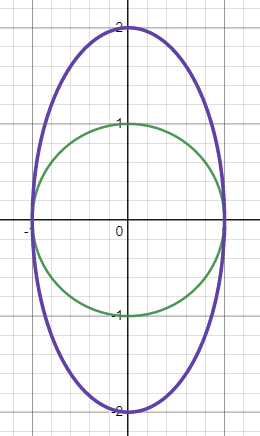
\includegraphics[scale=0.75]{fig1}
        \centering
        \caption{Two sample trajectories in $(q,p)$ space.}
        \label{fig1}
    \end{figure}

    \item Let's go the easy way first:
    \begin{align*}
        \poissonbracket{q}{p}_{(Q,P)} &= \pdv{q}{Q}\pdv{p}{P} - \pdv{q}{P}\pdv{p}{Q} \\
        &= \left(\sqrt{\frac{2P}{m\omega}}\cos Q\right)\left(\sqrt{\frac{m\omega}{2P}}\cos Q\right) - \left(\frac{1}{\sqrt{2Pm\omega}}\sin Q\right)\left(-\sqrt{2Pm\omega}\sin Q\right) \\
        &= \cos^2 Q + \sin^2 Q \\
        &= 1
    \end{align*}
    Now the other way! When we invert the transformation, we find
    \[ Q = \tan^{-1}(\frac{m\omega q}{p}); \quad P = \frac{p^2}{2m\omega} + \frac{1}{2}m\omega q^2. \]
    Now,
    \begin{align*}
        \poissonbracket{Q}{P}_{(q,p)} &= \pdv{Q}{q}\pdv{P}{p} - \pdv{Q}{p}\pdv{P}{q} \\
        &= \left(\frac{m\omega/p}{\left(\frac{m\omega q}{p}\right)^2 + 1}\right)\left(\frac{p}{m\omega}\right) - \left(-\frac{m\omega q}{\left(m \omega q\right)^2 + p^2}\right)\left(m\omega\right) \\
        &= \frac{p^2}{m^2\omega^2q^2 + p^2} + \frac{m^2\omega^2q^2}{m^2\omega^2q^2 + p^2} \\
        &= 1
    \end{align*}

    \item In the new coordinates, the hamiltonian is simply
    \[ H = \omega P\cos^2 Q + \omega P\sin^2 Q = \omega P. \]
    Hamilton's equations then give
    \[ \dot{P} = 0; \quad \dot{Q} = \omega, \]
    with general solutions
    \[ P(t) = P_0; \quad Q(t) = \omega t + Q_0 \]
    The resulting trajectories in phase space are just horizontal lines, as seen in Figure 2.
    \begin{figure}[H]
        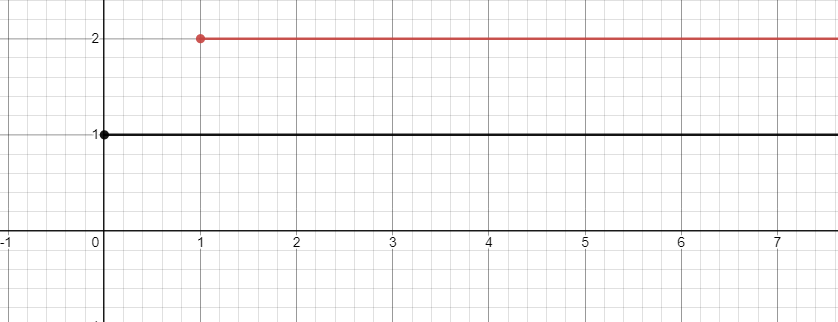
\includegraphics[scale=0.6]{fig2}
        \centering
        \caption{Two sample trajectories in $(Q,P)$ space.}
        \label{fig2}
    \end{figure}
\end{enumerate}


\end{document}